\chapter{Control Strategies and State Estimation} \label{ch:controlandestimation}
This project seeks to evaluate control strategies designed for a quadrotor, test its performance in simulation, and then implement them in the smartphone-based quadrotor prototype. In this chapter, the design procedure of the control and estimation algorithms for the quadrotor is shown. This algorithms are based on the linearized model of the quadrotor, detailed in Section \ref{sec:linearized}. Also, all the simulations carried out in MATLAB to verify the proper functioning of the designed algorithms are exposed.
\\\\
The state-space representation of the system, and the concept of controllability and observability, are briefly introduced in Section \ref{sec:generalities}. Then, Section \ref{sec:controlstrategies} shows the theoretical basis required for the design of the controllers used in this project. This controllers are the Linear Quadratic Integral (LQI) controller and the $H_\infty$ controller.
\\\\
Section \ref{sec:controldesign} presents the considerations made for the design of the two types of controllers according to the flight mode of the quadrotor. In addition, this section shows the simulated response of the quadrotor being controlled by both types of controllers in each flight mode.
\\\\
Finally, the state estimation algorithm developed mainly for the case of the LQI controller, is detailed in Section \ref{sec:stateestimation}.

\section{Concept and Generalities}
\label{sec:generalities}

\subsection{State Space Representation}
Recalling from Section \ref{sec:linearized}, the dynamic model of the quadrotor, based on its six $DoF$, is represented by the linear state-space model
\begin{align}
\label{ec:statespace}
\begin{split}
\dot{\mathbf{x}}(t) & = A\mathbf{x}(t)+B\mathbf{u}(t),\\[10px]
\mathbf{y}(t) & = C\mathbf{x}(t)+D\mathbf{u}(t),
\end{split}
\end{align}
where $A$ is the system matrix; $B$ is the input matrix; $C$ is the output matrix; $D$ is the feed-through matrix; $\mathbf{x}$ is the states vector of size $\mathit{n_x}$; $\mathbf{u}$ is the inputs vector of size $\mathit{n_u}$; and $\mathbf{y}$ is the outputs vector of size $\mathit{n_y}$.
\\\\
For simplicity, the state-space model representation shown in (\ref{ec:statespace}), can be represented by the quartet of matrices $\mathcal{G}$ as
\begin{equation}\label{eqn:ss}
\mathcal{G} = \mleft[
\begin{array}{c|c}
  A & B \\
  \hline
  C & D
\end{array}
\mright],
\end{equation}
while the discretized state-space model $\mathcal{G}_k$, using a sample time of $t_k$, is represented by
\begin{align}
\label{ec:statespace}
\begin{split}
\mathbf{x}(k+1) & = A_k\mathbf{x}(k)+B_k\mathbf{u}(k),\\[10px]
\mathbf{y}(k+1) & = C_k\mathbf{x}(k)+D_k\mathbf{u}(k).
\end{split}
\end{align}
Thus, $\mathcal{G}_k$ is represented by the quartet
\begin{equation}\label{eqn:ssk}
\mathcal{G}_k = \mleft[
\begin{array}{c|c}
  A_k & B_k \\
  \hline
  C_k & D_k
\end{array}
\mright],
\end{equation}
For the design of each controller, only the dynamics that are required to control, according to the flight mode in which the quadrotor is set, are taken into account. Therefore, system $\mathcal{G}$ will vary for each flight mode.

\subsection{Controllability and Observability}
The concept of controllability is related to the question of whether or not there exists a sequence of $\mathbf{u}$ capable of changing the states $\mathbf{x}$ from an initial value $\mathbf{x_0}$, to a desired final value $\mathbf{x_f}$, in a finite time. On the other hand, observability refers to the possibility of inferring, in finite time, the initial value of the states $\mathbf{x_0}$ knowing just the system dynamics $\mathcal{G}$ and its outputs $\mathbf{y}$ \cite{controlability1981}.
\\\\
Typically, the controllability and observability of a system are determined using the so-called controllability and observability matrices, $\mathcal{C_{G}}$ and $\mathcal{O_{G}}$ respectively.
This matrices depend on the system matrices $A$, $B$ and $C$, and are set as
\begin{align}
\begin{split}
\mathcal{C_{G}} & =
\begin{bmatrix}
B &  AB & \hdots & A^{k-1}B
\end{bmatrix},\\[5px]
\mathcal{O_G} & = \begin{bmatrix}
C\\
CA\\
\vdots\\
CA^{k-1}
\end{bmatrix}.
\end{split}
\end{align}
Thus, the system $\mathcal{G}$ is defined as controllable if $\mathcal{C_G}$ have $\mathit{n_x}$ linear independent rows (or columns). This is, the rank of $\mathcal{C_G}$ is equal to $\mathit{n_x}$. Analogous to the controllability, the observability of $\mathcal{G}$ is checked if the rank of the matrix $\mathcal{O_G}$ is equal to $\mathit{n_x}$.
\\\\
Another way to check the controllability and observability features of $\mathcal{G}$ is using the controllability and observability Grammians $\mathcal{W}_{c}$ and $\mathcal{W}_{o}$ defined as the solutions to the Lyapunov equations
\begin{align}
\begin{split}
0 & = A\mathcal{W}_{c} + \mathcal{W}_{c}A^{T} + BB^{T},\\[5px]
0 & = A^{T}\mathcal{W}_{o} + \mathcal{W}_{o}A + C^{T}C,
\end{split}
\end{align}
where
\begin{align}
\begin{split}
\mathcal{W}_{c} & = \int_{0}^{\infty}e^{At}BB^{T}e^{A^{T}t}dt,\\[5px]
\mathcal{W}_{o} & = \int_{0}^{\infty}e^{A^{T}t}C^{T}Ce^{At}dt.
\end{split}
\end{align}
In this case, if the matrices $\mathcal{W}_{c}$ and $\mathcal{W}_{o}$ are positive definite, the system is both controllable and observable \cite{Werner2012}.

\section{Control Strategies}
\label{sec:controlstrategies}
This section exposes the controllers design procedure. Here, the mathematical procedure to design a linear quadratic integral controller is described. It includes a regulator and an estimator, in addition to a gain compensator, allowing the system to track a trajectory. The design process of a $H_{\infty}$ controller is shown, taking into account some weighting sensitivities.

\subsection{Linear Quadratic Integral (LQI) Controller}
\subsubsection{Optimal Problem Solution}
The design of optimal controllers seeks that a dynamic system can be controlled achieving a minimum cost. The cost function is determined by the control designer \cite{Steinbuch2007}. Designing an finite-time regulator, a linear quadratic regulator (LQR) is set while looking for the minimization of the cost function $\mathcal{V}$ as
\begin{equation}
\mathcal{V} = \int_{0}^{T}\mathcal{L}(\mathbf{x},\mathbf{u},t)\ dt + \Psi(\mathbf{x},\mathbf{u},t),
\end{equation}
where
\begin{align}
\begin{split}
\mathcal{L}(\mathbf{x},\mathbf{u},t) = \mathbf{x}^{T}\mathcal{Q}\mathbf{x} + \mathbf{u}^{T}\mathcal{R}\mathbf{u},\\[5px]
\Psi(\mathbf{x},\mathbf{u},t) = \mathbf{x}^{T}(T)\mathcal{S}\mathbf{x}(T),
\end{split}
\end{align}
$\mathcal{R}$ is a positive definite matrix; and $\mathcal{Q}$ and $\mathcal{S}$ are positive semi-definite matrices. These matrices penalize the inputs, states and the terminal cost, respectively. Thus, the optimal controller design problem turns into an optimization problem where it is necessary to find an input $\mathbf{u}^{*}$ such that minimizes $\mathcal{V}$ for a controllable system subject to
\begin{align}
\begin{split}
\dot{\mathbf{x}}(t) & = \mathbf{f}(\mathbf{x}, \mathbf{u}, t) \approx A\mathbf{x}(t)+B\mathbf{u}(t),\\[5px]
\mathbf{x}(0) & = \mathbf{x_0},\ \ \ t \in [0, T].
\end{split}
\end{align}
This minimization is achieved using the Pontryagin maximum principle \cite{Murray2009}, where
\begin{equation}
\mathcal{H}(\mathbf{x},\mathbf{u},\lambda_\mathcal{P},t) = \mathcal{L}(\mathbf{x},\mathbf{u},t) + \lambda_\mathcal{P}^{T}\mathbf{f}(\mathbf{x}, \mathbf{u}, t)
\end{equation}
is the Hamiltonian function, with $\lambda_\mathcal{P}$ being the vector of co-state variables of size $\mathit{n_x}$, and
\begin{align}
\label{eqn:hamilt}
\begin{split}
\dot{\mathbf{x}}(t) & = \left(\dfrac{\partial \mathcal{H}(\mathbf{x},\mathbf{u},\lambda_\mathcal{P},t)}{\partial \lambda_\mathcal{P}}\right)^{T} = A\mathbf{x}(t)+B\mathbf{u}(t),\\[5px]
-\dot{\lambda}_{\mathcal{P}}(t) & = \left(\dfrac{\partial \mathcal{H}(\mathbf{x},\mathbf{u},\lambda_\mathcal{P},t)}{\partial \mathbf{x}}\right)^{T} = \mathcal{Q}\mathbf{x}(t) + A^{T}\lambda_{\mathcal{P}}(t),\\[5px]
0 & = \dfrac{\partial \mathcal{H}(\mathbf{x},\mathbf{u},\lambda_\mathcal{P},t)}{\partial \mathbf{u}} = \mathcal{R}\mathbf{u}(t) + \lambda_\mathcal{P}^{T}(t)B.
\end{split}
\end{align}
Thereby, from (\ref{eqn:hamilt}), the optimal solution to $\mathbf{u}$ that minimizes $\mathcal{H}(\mathbf{x},\mathbf{u},\lambda_\mathcal{P},t)$, and by Pontryagin maximum principle, the cost function $\mathcal{V}$, is
\begin{equation}
\mathbf{u}^{*}(t) = -\mathcal{R}^{-1}B^{T}\lambda_\mathcal{P}(t).
\end{equation}
Assuming that $\lambda_\mathcal{P}(t) = \mathcal{P}(t)\mathbf{x}(t)$, the optimal input $\mathbf{u}^{*}$ depends directly on a feedback vector, which is the state vector $\mathbf{x}$, such that
\begin{align}
\label{eqn:optimalu}
\begin{split}
\mathbf{u}^{*}(t) & = \mathbf{K_{lqr}}(t)\mathbf{x}(t),\\[5px]
\mathbf{K_{lqr}}(t) & = -\mathcal{R}^{-1}B^{T}\mathcal{P}(t).
\end{split}
\end{align}
Here, matrix $\mathcal{P}(t)$ is a solution of the Riccati Equation \cite{Moore1989}
	\begin{equation}
	-\dot{\mathcal{P}} = \mathcal{P}A + A^{T}\mathcal{P} + \mathcal{Q} - \mathcal{P}B\mathcal{R}^{-1}B^{T}\mathcal{P}.
	\end{equation}
When $T \to \infty$, an infinite-time regulator is designed. Here, aiming for a steady-state solution, the terminal cost $\Psi(\mathbf{x}, \mathbf{u},t)$ is eliminated, and the matrix $\mathcal{P}$ is assumed to be constant. Thus, $\mathcal{P}$ is a solution of the Algebraic Riccati Equation (ARE)
	\begin{equation}
	0 = \mathcal{P}A + A^{T}\mathcal{P} + \mathcal{Q} - \mathcal{P}B\mathcal{R}^{-1}B^{T}\mathcal{P}.
	\end{equation}
Consequently, in the infinite-time LQR, the optimal input $\mathbf{u}^{*}$ is achieved by multiplying the state vector $\mathbf{x}$ with the constant feedback gain matrix
\begin{equation}
\mathbf{K_{lqr}} = -\mathcal{R}^{-1}B^{T}\mathcal{P}.
\end{equation}
\\As the feedback gain is not a dynamical system, but a static matrix, the order of the closed-loop dynamics is the same as the one of the system dynamics $\mathcal{G}$. The closed-loop dynamics are written as
\begin{equation}
\dot{\mathbf{x}} = (A+B\mathbf{K_{lqr}})\mathbf{x}.
\end{equation}
When the desired state value $\mathbf{x_{des}}$ is different from zero, these reference value is applied to the dynamics through the feedback gain matrix as
\begin{equation}
\dot{\mathbf{x}} = (A+B\mathbf{K_{lqr}})\mathbf{x}-B\mathbf{K_{lqr}}\mathbf{x_{des}},
\end{equation}
due to the fact that the error $\mathbf{e_x} = \mathbf{x} - \mathbf{x_{des}}$ is used as the feedback vector of the LQR.

\subsubsection{Reference Tracking}
For the quadrotor position control, a controller capable of reference tracking is necessary. However, the LQR controller is not made for reference tracking, but just for regulation. This is overcame making use of a Linear Quadratic Integral (LQI) controller, which is a LQR with an additional integral feedback. The integral action ensures that a zero steady-state error is achieved. 
\\\\
The approach of using integral feedback with a LQR to provide tracking capabilities to the control system, is based on the augmentation of the state vector $\mathbf{x}$ with a vector
\begin{equation}
\mathbf{x_i} = \int \mathbf{e}\ dt,\ \ \mathbf{x_i}(0) = \mathbf{0},\ \ \mathbf{x_i} \in \mathbb{R}^{n_y},
\end{equation}
containing the integral of the error signal $\mathbf{e} = r - \mathbf{y}$, where $r$ is the reference signal of size $n_y$. The augmented state vector $\mathbf{x_{lqi}}$ is defined as
\begin{equation}
\mathbf{x_{lqi}} = \begin{bmatrix}
\mathbf{x} \\
\mathbf{x_i}
\end{bmatrix},
\end{equation}
with which the augmented system to be controlled is obtained as
\begin{align}
\label{eqn:augmentedLQI}
\begin{split}
\mathbf{\dot{x}_{lqi}} & = \bar{A}\mathbf{x_{lqi}} + \bar{B}\mathbf{u} + B_{i}r,\\[5px]
\mathbf{y} & = \bar{C}\mathbf{x_{lqi}},
\end{split}
\end{align}
where
\begin{align}
\begin{split}
\bar{A} & = \begin{bmatrix}
A & \mathbf{0_{\mathit{n_x}\times \mathit{n_y}}} \\
-C & \mathbf{0_{\mathit{n_y}\times \mathit{n_y}}}
\end{bmatrix}, \\[5px]
\bar{B} & = \begin{bmatrix}
B \\ \mathbf{0_{\mathit{n_y}\times \mathit{n_u}}}
\end{bmatrix}, \\[5px]
B_{r} & = \begin{bmatrix}
\mathbf{0_{\mathit{n_x}\times \mathit{n_y}}} \\
\mathcal{I}_{\mathit{n_y}\times \mathit{n_y}}
\end{bmatrix}, \\[5px]
\bar{C} & = \begin{bmatrix}
C & \mathbf{0_{\mathit{n_y}\times \mathit{n_y}}}
\end{bmatrix}.
\end{split}
\end{align}
Given the augmented system in (\ref{eqn:augmentedLQI}), the controller is designed using the Optimal Problem Solution detailed before, obtaining a control law of the form
\begin{align}
\begin{split}
\mathbf{u} & = \mathbf{K_{lqi}}\mathbf{x_{lqi}} =\begin{bmatrix}
\mathbf{K_{lqr}} & \mathbf{K_{i}}
\end{bmatrix}\begin{bmatrix}
\mathbf{x} \\
\mathbf{x_i}
\end{bmatrix},
\end{split}
\end{align}
where $\mathbf{K_{lqr}}$ and $\mathbf{K_i}$ are  submatrices which correspond to the feedback gain matrices that multiply $\mathbf{x}$ and $\mathbf{x_i}$ respectively, as shown in Fig. \ref{fig:lqi}.
	\begin{figure}[h]
	\begin{center}
	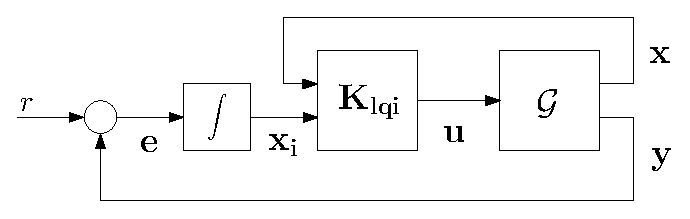
\includegraphics[width=10.5cm]{lqi}
	\caption{Closed-loop system with LQI controller for reference tracking}
	\label{fig:lqi}
	\end{center}
	\end{figure}


\subsection{$H_\infty$ Controller}
\subsubsection{$H_\infty$ Synthesis for Controller Design}
The design of the $H_\infty$ controller is based on a representation of the closed-loop system including the generalized plant $P_H$ and the controller $K_H$, shown in Fig. \ref{fig:generalized}.
	\begin{figure}[h]
	\begin{center}
	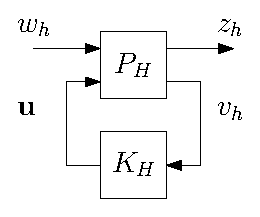
\includegraphics[width=4.5cm]{generalized}
	\caption{Control loop with generalized plant}
	\label{fig:generalized}
	\end{center}
	\end{figure}
\\\\The generalized plant $P_H$ corresponds to the system
\begin{align}
\begin{split}
\mathbf{\dot{x}} & = A\mathbf{x} + B_{w}w_{h} + B\mathbf{u},\\[5px]
z_{h} & = C_{z}\mathbf{x} + D_{zw}w_{h} + D_{zu}\mathbf{u},\\[5px]
v_{h} & = -C\mathbf{x} + D_{vw}w_{h} + D_{vu}\mathbf{u}.
\end{split}
\end{align} 
where $w_h$ are the external inputs, including command inputs, disturbances and noises; $z_h$ is a fictitious output vector used to express design specifications; and $v_h$ are the measured outputs of the system \cite{Werner2012}.
\\\\
The $H_\infty$ design procedure aims to synthesize a dynamic controller $K_H$, with input $v_h = -\mathbf{y}$ and output $\mathbf{u}$, such that the closed-loop system is stabilized and the fictitious output $z_h$ is minimized.
\\\\
The system in Fig. \ref{fig:generalized}, is rearranged for easy interpretation, in the way of Fig. \ref{fig:augmentedPlant}.
\begin{figure}[h]
	\begin{center}
	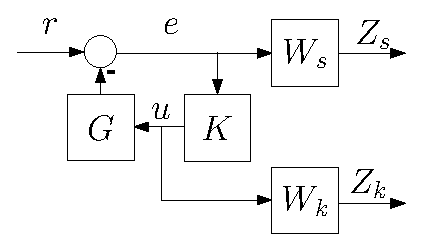
\includegraphics[width=6.5cm]{augmentedPlant.eps}
	\caption{Generalized plant with the weighting filters $W_s$ and $W_k$.}
	\label{fig:augmentedPlant}
	\end{center}
	\end{figure}	
\\In Fig. \ref{fig:augmentedPlant}, $\mathcal{G}$ represents the quadrotor dynamics; $K_H$ the controller; $r$ is the system reference; $\mathbf{e}$ is the error; $\mathbf{u}$ is the control input; $z_{h} = \begin{bmatrix}
Z_s & Z_k
\end{bmatrix}$; and $W_{s},\ W_{k}$ are weighting filters that must satisfy 
	\begin{equation}\label{eqn:hinf}
	\gamma = \left|\left|\begin{bmatrix}
	W_{s}S\\W_{k}KS
	\end{bmatrix}\right|\right|_{\infty} < 1,
	\end{equation}
\\where $S$ is the sensitivity function and $K_{H}S$ is the control sensitivity defined as
	\begin{equation}
	S = (\mathcal{I} + \mathcal{G}K_{H})^{-1},\ \ \ K_{H}S = K_{H}(\mathcal{I} + \mathcal{G}K_{H})^{-1}.
	\end{equation}
The $H_\infty$ norm is defined only for proper and stable systems, so the weighting filters must satisfy that condition. The weighting filter $W_{s}$ impose an upper bound on the sensitivity and is designed taking into account that it is desired to have integral action in the closed-loop. This ensures a zero steady-state error. On the other hand, the filter $W_k$ impose an upper bound on the control sensitivity and must have a high-pass behaviour.
\\\\
The weighting filters for the sensitivity and the control sensitivity are chosen as
\begin{align}\label{eqn:wswk}
\begin{split}
W_{s} &= \dfrac{w_{s}/M_{s}}{s + w_{s}}*\mathcal{I}_{n_{y}\times n_{y}}\ ,\\
W_{k} &= \dfrac{c_k}{M_{k}}\dfrac{s+w_{k}}{s+c_{k}w_{k}}*\mathcal{I}_{n_{u}\times n_{u}}\ ,
\end{split}
\end{align}
where $M_s$ is small constant that sets an upper bound on the sensitivity at low frequencies; and $w_s$ is a small constant that ensures that $W_s$ does not have a pole at the origin; $M_k$ is a constant that sets the upper bound on the control sensitivity at low frequencies; $w_k$ is a small constant that place the zero of $W_k$ near the origin; and $c_k$ is a large constant that place the pole of $W_k$ at a frequency above the bandwidth.
\\\\
If the resulting value of $\gamma$ is greater than one, the design procedure is iterated normalizing the weighting filters with $\gamma$.
\\\\
In this project, the synthesized optimal $H_\infty$ controllers $K_H$ are computed using the Robust Control Toolbox of MATLAB.

\subsubsection{$H_\infty$ Controller Order Reduction}
The designed $H_{\infty}$ controller $K_H$ is a dynamic model with $n_u$ outputs, $n_y$ inputs and
order $n_H = n_{x} + n_{y} + n_{u}$. To reduce the computational load that the execution of a high-order dynamic system entails, it is necessary to find a reduced order controller that behaves similarly to the full order controller $K_H$. 
\\\\
In a dynamic system, the states with small singular value energy in $\mathcal{W}_{c}$ show a weak response to a control input, while states with small singular value energy in $\mathcal{W}_{o}$ have weak influence on the observed output. In order to check which states of $K_H$ have little influence both in terms of controllability and observability, the singular values of the Hankel matrix
\begin{equation}
H_{k} = \mathcal{O_{K_H}}\mathcal{C_{K_H}},
\end{equation}
are analysed. The matrices $\mathcal{C_{K_H}}$ and $\mathcal{O_{K_H}}$ represent the controllability and observability matrices of the system $K_H$, respectively. A Hankel singular value (HSV) with small energy indicates that a state has little influence both in terms of controllability and observability.
\\\\
If $\hat{K}_{H}=(\hat{A}_H,\ \hat{B}_H,\ \hat{C}_H,\ \hat{D}_H)$ is the balanced realization of $K_H$ with $n_H$ state variables, and we have $n_h$ significant states, so the last $n_{H}-n_{h}$ HSVs are small enough to be neglected without modifying the system dynamics \cite{Skogestad2005}. 

\section{Controllers Design and Simulation}
\label{sec:controldesign}
fhfgfhfh
\subsection{Stabilize Mode}
fghgfh
\subsubsection{Dynamic Model}
\begin{align}
\begin{split}
\mathbf{x} = & \begin{bmatrix}
\psi & \dot{\psi} & \theta & \dot{\theta} & \phi & \dot{\phi}
\end{bmatrix}^{T},\\[15px]
\mathbf{y} = & \begin{bmatrix}
\psi & \theta & \phi
\end{bmatrix}^{T}
\end{split}
\end{align}
\begin{align}
\begin{split}
A = & 
\begin{bmatrix}
0 & 1 & 0 & 0 & 0 & 0 \\[2px]
0 & 0 & 0 & 0 & 0 & 0 \\[2px]
0 & 0 & 0 & 1 & 0 & 0 \\[2px]
0 & 0 & 0 & 0 & 0 & 0 \\[2px]
0 & 0 & 0 & 0 & 0 & 1 \\[2px]
0 & 0 & 0 & 0 & 0 & 0
\end{bmatrix}, \\[15px]
B = & 
\begin{bmatrix}
0 & 0 & 0 & 0 & 0 & 0\\[5px]
0 & \dfrac{1}{J_{zz}} & 0 & 0 & 0 & 0\\[5px]
0 & 0 & 0 & \dfrac{1}{J_{yy}} & 0 & 0\\[5px]
0 & 0 & 0 & 0 & 0 & \dfrac{1}{J_{xx}}
\end{bmatrix}^{T}.
\end{split}
\end{align}
\begin{align}
\begin{split}
C = & 
\begin{bmatrix}
1 & 0 & 0 & 0 & 0 & 0 \\[2px]
0 & 0 & 1 & 0 & 0 & 0 \\[2px]
0 & 0 & 0 & 0 & 1 & 0
\end{bmatrix}, \\[15px]
D = &\ \mathbf{0_{3\times 4}}.
\end{split}
\end{align}
\subsubsection{Linear Quadratic Regulator}
rtrte

\begin{figure}[H]
\begin{subfigure}{.5\linewidth}
\centering
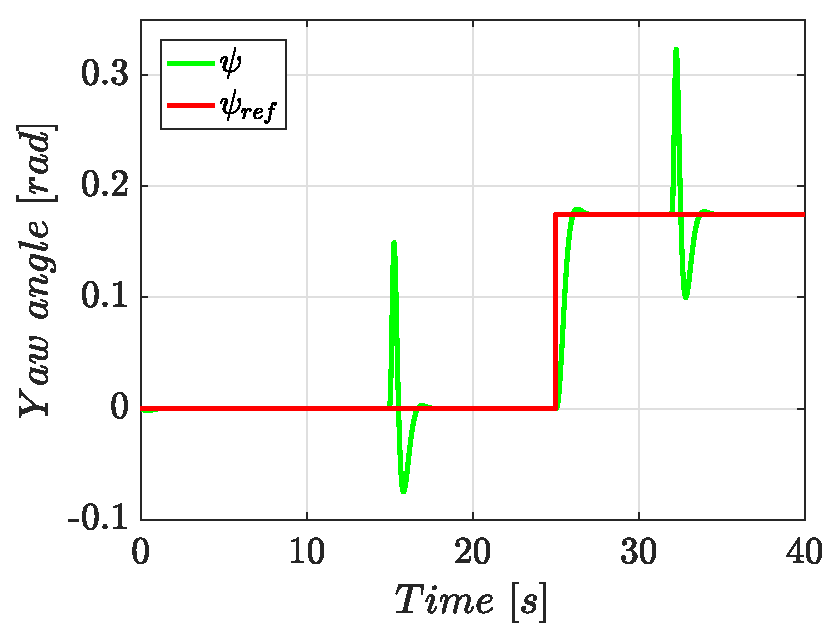
\includegraphics[width=7.0cm]{stabilize_psi_lqi}
\caption{Rotation about $x$ axis, $J_{xx}$ experiment}
\label{fig:stabilize_psi_lqi}
\end{subfigure}%
\begin{subfigure}{.5\linewidth}
\centering
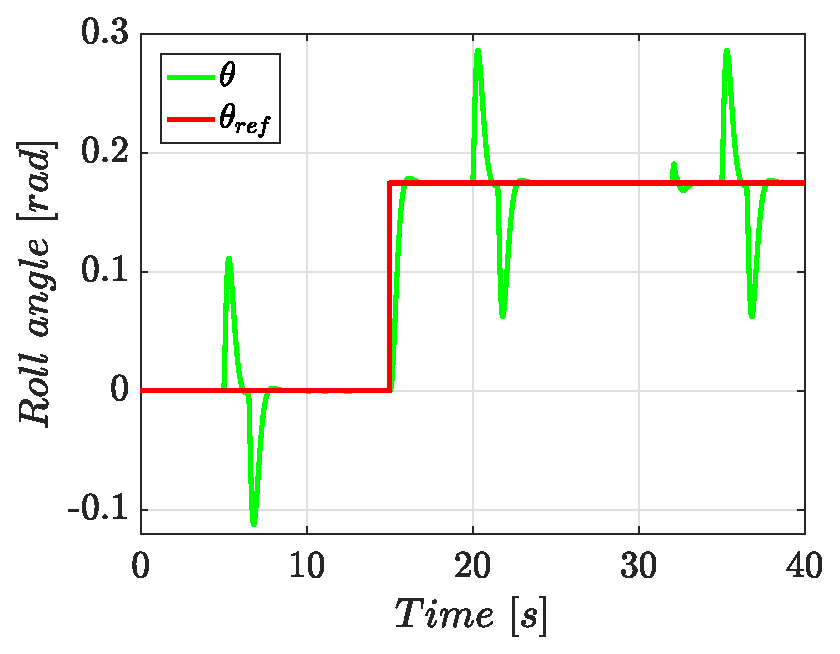
\includegraphics[width=7.0cm]{stabilize_theta_lqi}
\caption{Rotation about $y$ axis, $J_{yy}$ experiment}
\label{fig:stabilize_theta_lqi}
\end{subfigure}\\[1ex]
\begin{subfigure}{\linewidth}
\centering
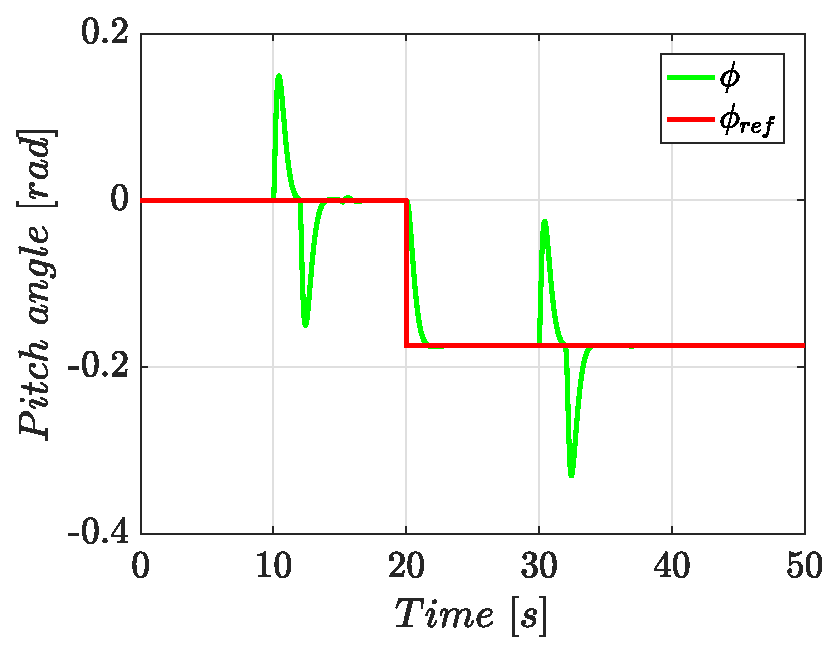
\includegraphics[width=7.0cm]{stabilize_phi_lqi}
\caption{Rotation about $z$ axis, $J_{zz}$ experiment}
\label{fig:stabilize_psi_lqi}
\end{subfigure}
\caption{Rotation about $x$, $y$ and $z$ axes during the bifilar pendulum experiments}
\label{fig:stabilize_lqi}
\end{figure}

\subsubsection{$H_\infty$ Controller}
rtrtererre
$\gamma = 0.0150$

where $w_{s} = 10^{-4}$, $M_{s} = 10^{-4}$, $w_{k} = 20$, $M_{k} = 20$, and $c_{k} = 10^{3}$.

\begin{figure}[h]
\begin{center}
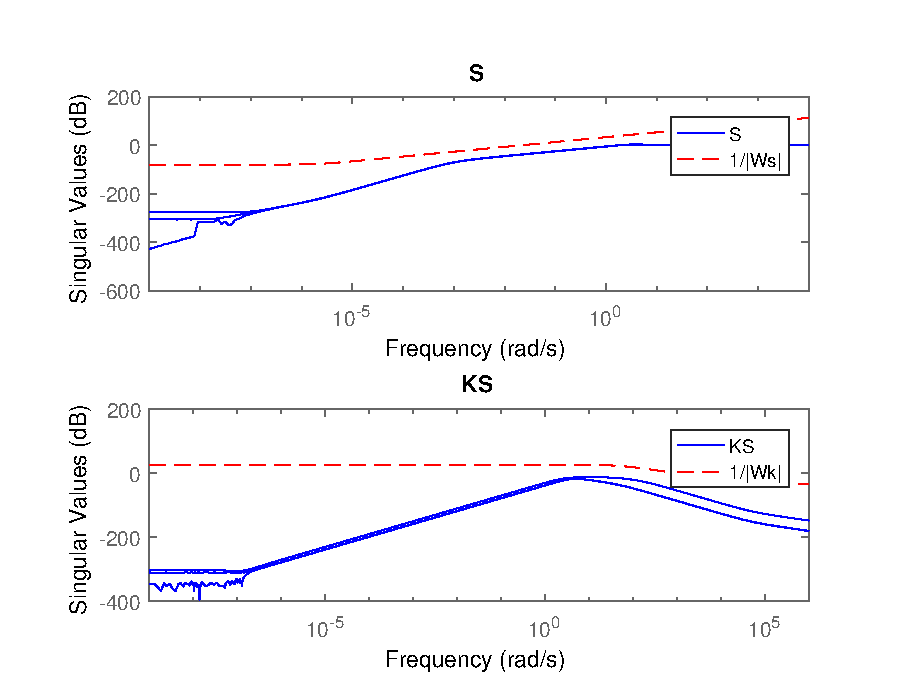
\includegraphics[width=10.8cm]{sv_stabilize_hinf}  
\caption{Hankel singular values energy histogram of the designed controller.} 
\label{fig:sv_stabilize_hinf}
\end{center}
\end{figure}
13 states, then 12
The energy of the  is shown in Fig. \ref{fig:hsv}.
\begin{figure}[h]
\begin{center}
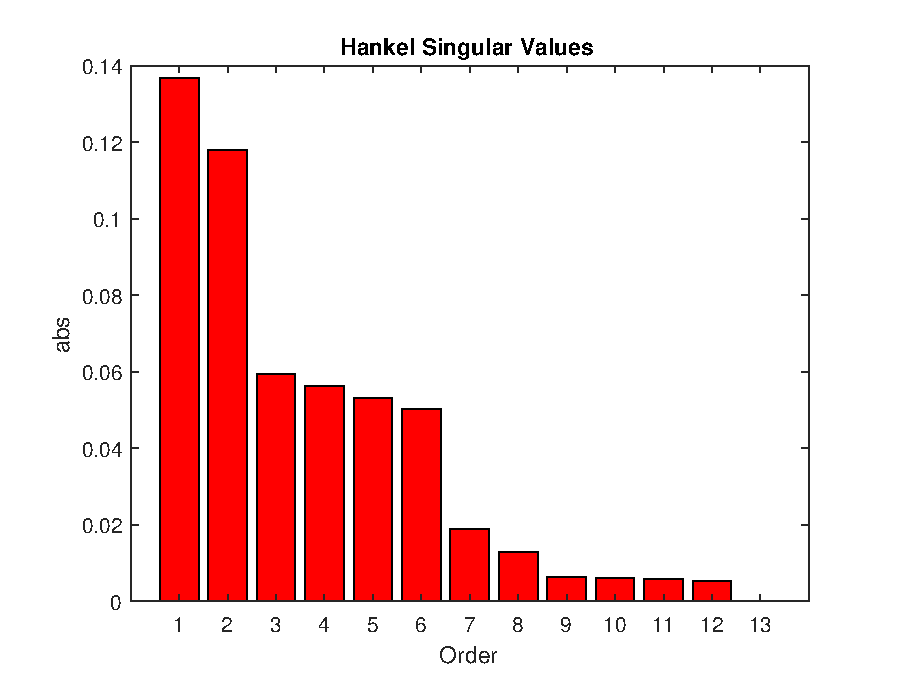
\includegraphics[width=10.8cm]{hsv_stabilize_h}  
\caption{Hankel singular values energy histogram of the designed controller.} 
\label{fig:hsv_stabilize_h}
\end{center}
\end{figure}
As shown in Fig. \ref{fig:hsv}, the last ordered four states have unnoticeable energy when it is plotted; that means that these four states can be truncated from the controller without modifying its dynamics.
\begin{figure}[H]
\begin{subfigure}{.5\linewidth}
\centering
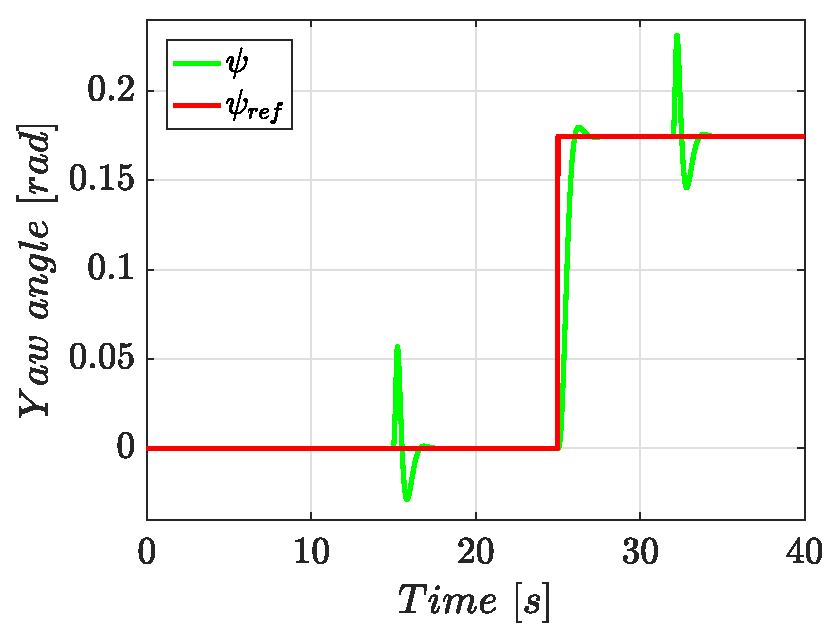
\includegraphics[width=7.0cm]{stabilize_psi_h}
\caption{Rotation about $x$ axis, $J_{xx}$ experiment}
\label{fig:stabilize_psi_h}
\end{subfigure}%
\begin{subfigure}{.5\linewidth}
\centering
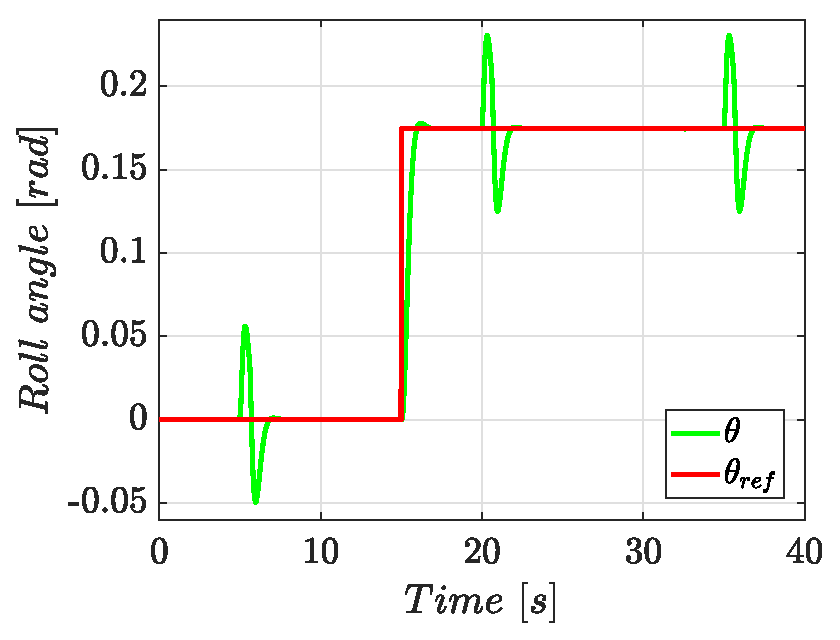
\includegraphics[width=7.0cm]{stabilize_theta_h}
\caption{Rotation about $y$ axis, $J_{yy}$ experiment}
\label{fig:stabilize_theta_h}
\end{subfigure}\\[1ex]
\begin{subfigure}{\linewidth}
\centering
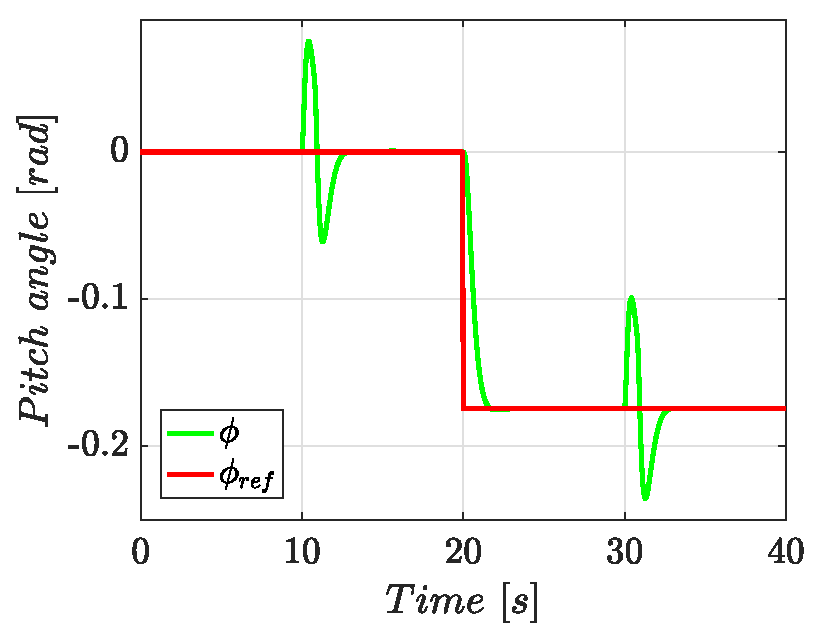
\includegraphics[width=7.0cm]{stabilize_phi_h}
\caption{Rotation about $z$ axis, $J_{zz}$ experiment}
\label{fig:stabilize_psi_h}
\end{subfigure}
\caption{Rotation about $x$, $y$ and $z$ axes during the bifilar pendulum experiments}
\label{fig:stabilize_lqi}
\end{figure}


\subsection{Altitude Hold Mode}
\subsubsection{Dynamic Model}

\begin{align}
\begin{split}
\mathbf{x} = & \begin{bmatrix}
z & \dot{z} & \psi & \dot{\psi} & \theta & \dot{\theta} & \phi & \dot{\phi}
\end{bmatrix}^{T},\\[15px]
\mathbf{y} = & \begin{bmatrix}
z & \psi & \theta & \phi
\end{bmatrix}^{T}
\end{split}
\end{align}
\begin{align}
\begin{split}
A = & 
\begin{bmatrix}
0 & 1 & 0 & 0 & 0 & 0 & 0 & 0\\[2px]
0 & 0 & 0 & 0 & 0 & 0 & 0 & 0\\[2px]
0 & 0 & 0 & 1 & 0 & 0 & 0 & 0\\[2px]
0 & 0 & 0 & 0 & 0 & 0 & 0 & 0\\[2px]
0 & 0 & 0 & 0 & 0 & 1 & 0 & 0\\[2px]
0 & 0 & 0 & 0 & 0 & 0 & 0 & 0\\[2px]
0 & 0 & 0 & 0 & 0 & 0 & 0 & 1\\[2px]
0 & 0 & 0 & 0 & 0 & 0 & 0 & 0
\end{bmatrix}, \\[15px]
B = & 
\begin{bmatrix}
0 & \dfrac{1}{m} & 0 & 0 & 0 & 0 & 0 & 0\\[5px]
0 & 0 & 0 & \dfrac{1}{J_{zz}} & 0 & 0 & 0 & 0\\[5px]
0 & 0 & 0 & 0 & 0 & \dfrac{1}{J_{yy}} & 0 & 0\\[5px]
0 & 0 & 0 & 0 & 0 & 0 & 0 & \dfrac{1}{J_{xx}}
\end{bmatrix}^{T}.
\end{split}
\end{align}
\begin{align}
\begin{split}
C = & 
\begin{bmatrix}
1 & 0 & 0 & 0 & 0 & 0 & 0 & 0 \\[2px]
0 & 0 & 1 & 0 & 0 & 0 & 0 & 0 \\[2px]
0 & 0 & 0 & 0 & 1 & 0 & 0 & 0 \\[2px]
0 & 0 & 0 & 0 & 0 & 0 & 1 & 0 
\end{bmatrix}, \\[15px]
D = &\ \mathbf{0_{4\times 4}}.
\end{split}
\end{align}
\subsubsection{Linear Quadratic Regulator}
rtrterere
\begin{figure}[H]
\begin{subfigure}{.5\linewidth}
\centering
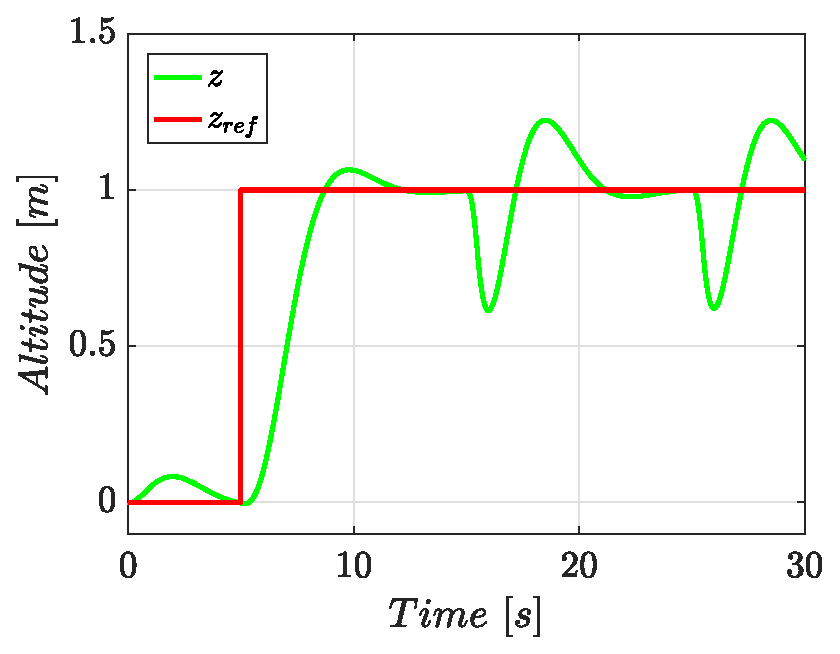
\includegraphics[width=7.0cm]{althold_z_lqi}
\caption{Rotation about $x$ axis, $J_{xx}$ experiment}
\label{fig:althold_z_lqi}
\end{subfigure}%
\begin{subfigure}{.5\linewidth}
\centering
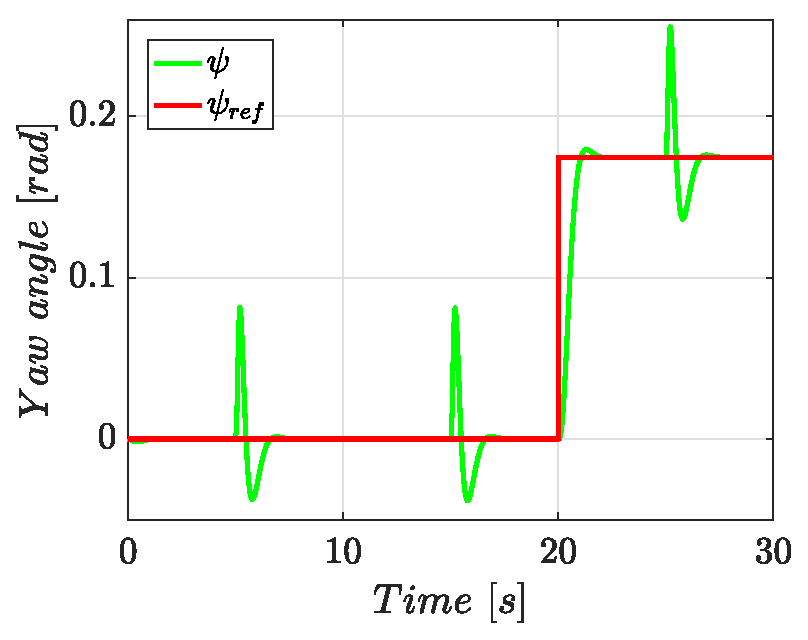
\includegraphics[width=7.0cm]{althold_psi_lqi}
\caption{Rotation about $y$ axis, $J_{yy}$ experiment}
\label{fig:althold_psi_lqi}
\end{subfigure}\\[1ex]
\begin{subfigure}{0.5\linewidth}
\centering
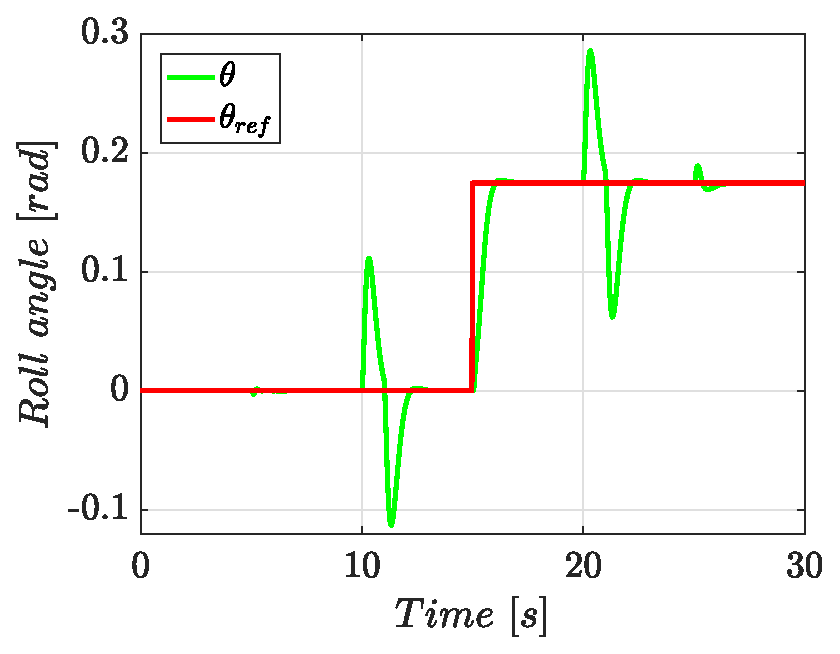
\includegraphics[width=7.0cm]{althold_theta_lqi}
\caption{Rotation about $z$ axis, $J_{zz}$ experiment}
\label{fig:althold_theta_lqi}
\end{subfigure}
\begin{subfigure}{0.5\linewidth}
\centering
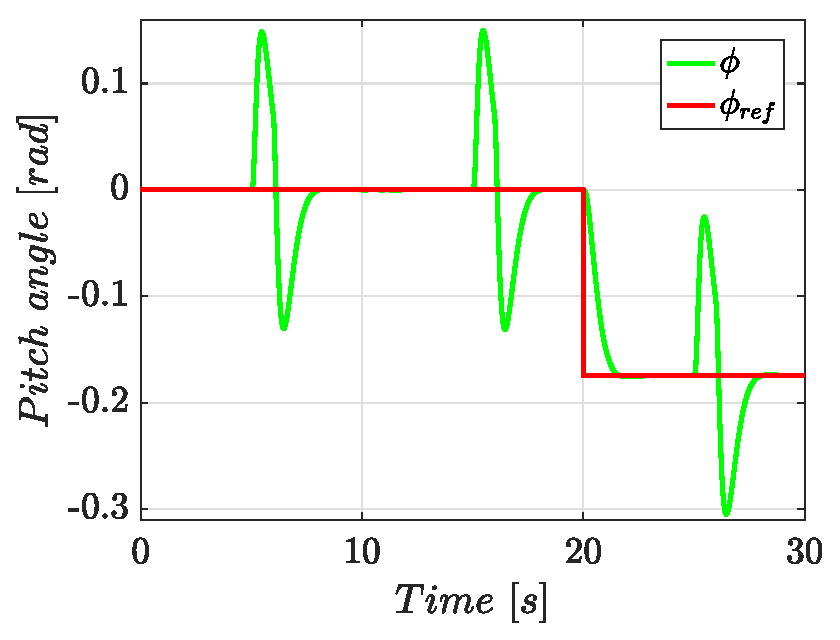
\includegraphics[width=7.0cm]{althold_phi_lqi}
\caption{Rotation about $z$ axis, $J_{zz}$ experiment}
\label{fig:althold_phi_lqi}
\end{subfigure}
\caption{Rotation about $x$, $y$ and $z$ axes during the bifilar pendulum experiments}
\label{fig:althold_lqi}
\end{figure}

\subsubsection{$H_\infty$ Controller}
rtrtererre
$\gamma = 0.5976$
\begin{figure}[h]
\begin{center}
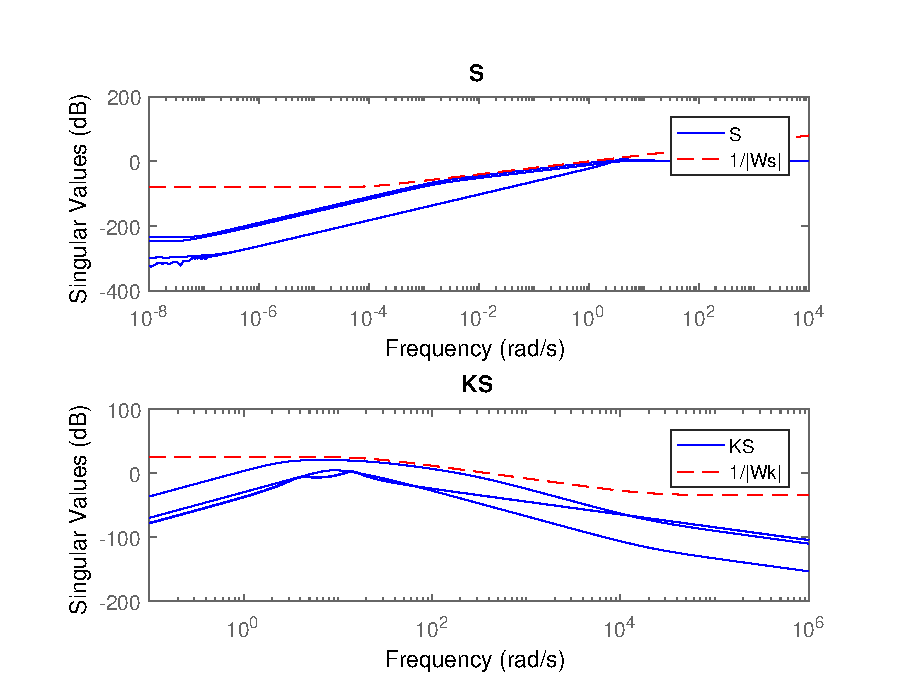
\includegraphics[width=10.8cm]{sv_althold_hinf}  
\caption{Hankel singular values energy histogram of the designed controller.} 
\label{fig:sv_auto_hinf}
\end{center}
\end{figure}
16 states, then 10
The energy of the  is shown in Fig. \ref{fig:hsv}.
\begin{figure}[h]
\begin{center}
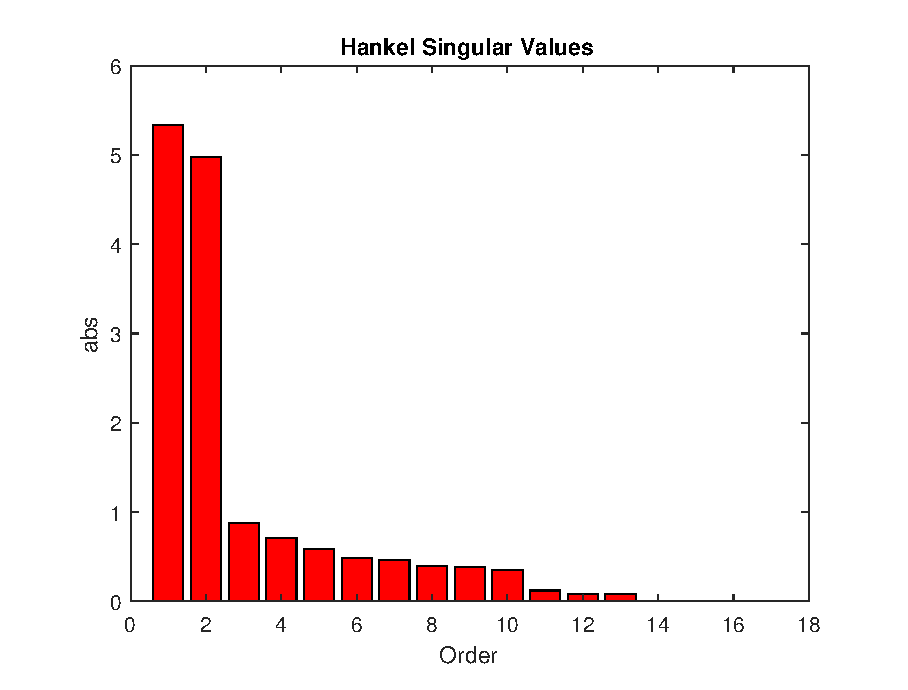
\includegraphics[width=10.8cm]{hsv_althold_h}  
\caption{Hankel singular values energy histogram of the designed controller.} 
\label{fig:hsv_auto_h}
\end{center}
\end{figure}
As shown in Fig. \ref{fig:hsv}, the last ordered four states have unnoticeable energy when it is plotted; that means that these four states can be truncated from the controller without modifying its dynamics.

\begin{figure}[H]
\begin{subfigure}{.5\linewidth}
\centering
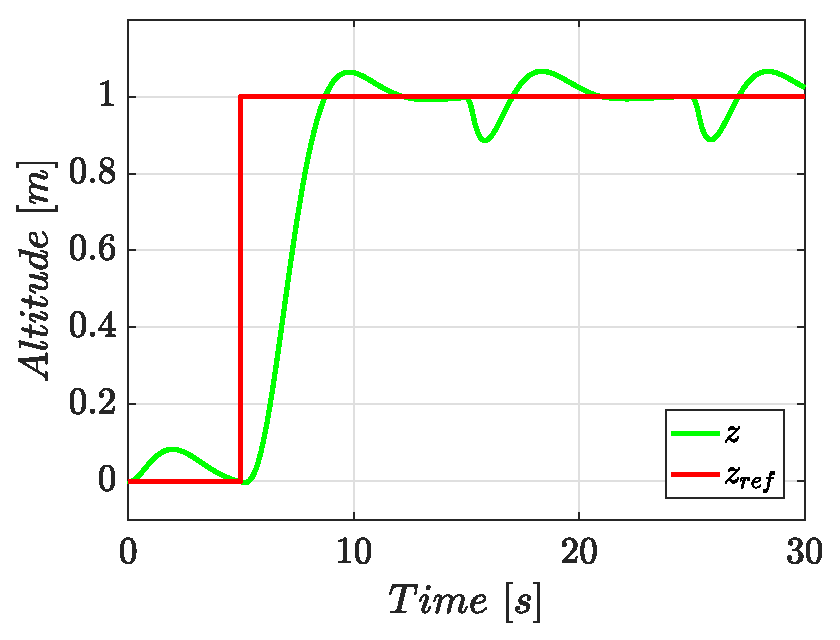
\includegraphics[width=7.0cm]{althold_z_h}
\caption{Rotation about $x$ axis, $J_{xx}$ experiment}
\label{fig:althold_z_h}
\end{subfigure}%
\begin{subfigure}{.5\linewidth}
\centering
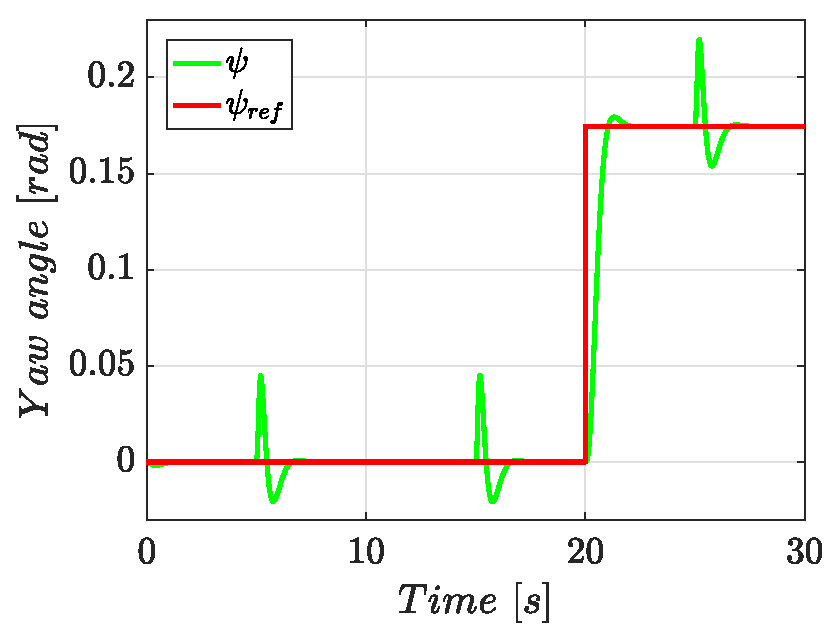
\includegraphics[width=7.0cm]{althold_psi_h}
\caption{Rotation about $y$ axis, $J_{yy}$ experiment}
\label{fig:althold_psi_h}
\end{subfigure}\\[1ex]
\begin{subfigure}{0.5\linewidth}
\centering
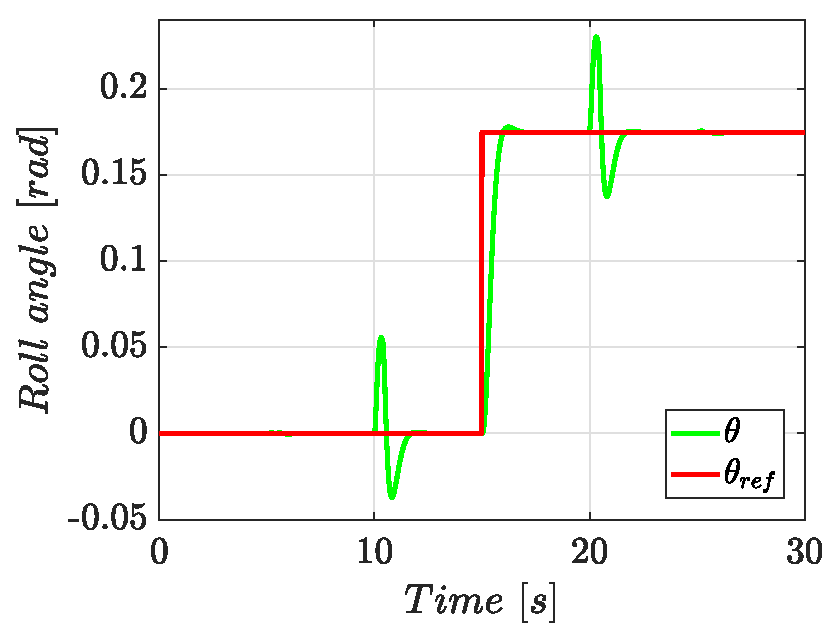
\includegraphics[width=7.0cm]{althold_theta_h}
\caption{Rotation about $z$ axis, $J_{zz}$ experiment}
\label{fig:althold_theta_h}
\end{subfigure}
\begin{subfigure}{0.5\linewidth}
\centering
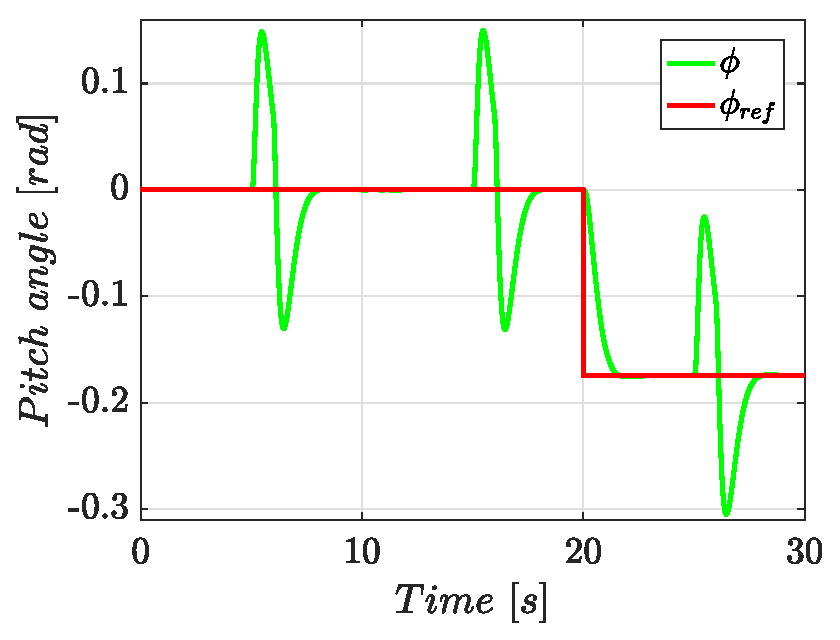
\includegraphics[width=7.0cm]{althold_phi_lqi}
\caption{Rotation about $z$ axis, $J_{zz}$ experiment}
\label{fig:althold_phi_h}
\end{subfigure}
\caption{Rotation about $x$, $y$ and $z$ axes during the bifilar pendulum experiments}
\label{fig:althold_h}
\end{figure}

\subsection{GNSS Dependent Flight Modes}

\subsubsection{Dynamic Model}
\begin{align}
\begin{split}
\mathbf{x} = & \begin{bmatrix}
x & \dot{x} & y & \dot{y} & z & \dot{z} & \psi & \dot{\psi} & \theta & \dot{\theta} & \phi & \dot{\phi}
\end{bmatrix}^{T},\\[15px]
\mathbf{y} = & \begin{bmatrix}
x & y & z & \psi & \theta & \phi
\end{bmatrix}^{T}
\end{split}
\end{align}

\begin{align}
\begin{split}
A = & 
\begin{bmatrix}
0 & 1 & 0 & 0 & 0 & 0 & 0 & 0 & 0 & 0 & 0 & 0\\[2px]
0 & 0 & 0 & 0 & 0 & 0 & 0 & 0 & g & 0 & 0 & 0\\[2px]
0 & 0 & 0 & 1 & 0 & 0 & 0 & 0 & 0 & 0 & 0 & 0\\[2px]
0 & 0 & 0 & 0 & 0 & 0 & 0 & 0 & 0 & 0 & g & 0\\[2px]
0 & 0 & 0 & 0 & 0 & 1 & 0 & 0 & 0 & 0 & 0 & 0\\[2px]
0 & 0 & 0 & 0 & 0 & 0 & 0 & 0 & 0 & 0 & 0 & 0\\[2px]
0 & 0 & 0 & 0 & 0 & 0 & 0 & 1 & 0 & 0 & 0 & 0\\[2px]
0 & 0 & 0 & 0 & 0 & 0 & 0 & 0 & 0 & 0 & 0 & 0\\[2px]
0 & 0 & 0 & 0 & 0 & 0 & 0 & 0 & 0 & 1 & 0 & 0\\[2px]
0 & 0 & 0 & 0 & 0 & 0 & 0 & 0 & 0 & 0 & 0 & 0\\[2px]
0 & 0 & 0 & 0 & 0 & 0 & 0 & 0 & 0 & 0 & 0 & 1\\[2px]
0 & 0 & 0 & 0 & 0 & 0 & 0 & 0 & 0 & 0 & 0 & 0
\end{bmatrix}, \\[15px]
B = & 
\begin{bmatrix}
0 & 0 & 0 & 0 & 0 & \dfrac{1}{m} & 0 & 0 & 0 & 0 & 0 & 0\\[5px]
0 & 0 & 0 & 0 & 0 & 0 & 0 & \dfrac{1}{J_{zz}} & 0 & 0 & 0 & 0\\[5px]
0 & 0 & 0 & 0 & 0 & 0 & 0 & 0 & 0 & \dfrac{1}{J_{yy}} & 0 & 0\\[5px]
0 & 0 & 0 & 0 & 0 & 0 & 0 & 0 & 0 & 0 & 0 & \dfrac{1}{J_{xx}}
\end{bmatrix}^{T}.
\end{split}
\end{align}
\begin{align}
\begin{split}
C = & 
\begin{bmatrix}
1 & 0 & 0 & 0 & 0 & 0 & 0 & 0 & 0 & 0 & 0 & 0 \\[2px]
0 & 0 & 1 & 0 & 0 & 0 & 0 & 0 & 0 & 0 & 0 & 0 \\[2px]
0 & 0 & 0 & 0 & 1 & 0 & 0 & 0 & 0 & 0 & 0 & 0 \\[2px]
0 & 0 & 0 & 0 & 0 & 0 & 1 & 0 & 0 & 0 & 0 & 0 \\[2px]
0 & 0 & 0 & 0 & 0 & 0 & 0 & 0 & 1 & 0 & 0 & 0 \\[2px]
0 & 0 & 0 & 0 & 0 & 0 & 0 & 0 & 0 & 0 & 1 & 0
\end{bmatrix}, \\[15px]
D = &\ \mathbf{0_{6\times 4}}.
\end{split}
\end{align}
\subsubsection{Linear Quadratic Regulator}
rtrterere
\begin{figure}[h]
	\begin{center}
	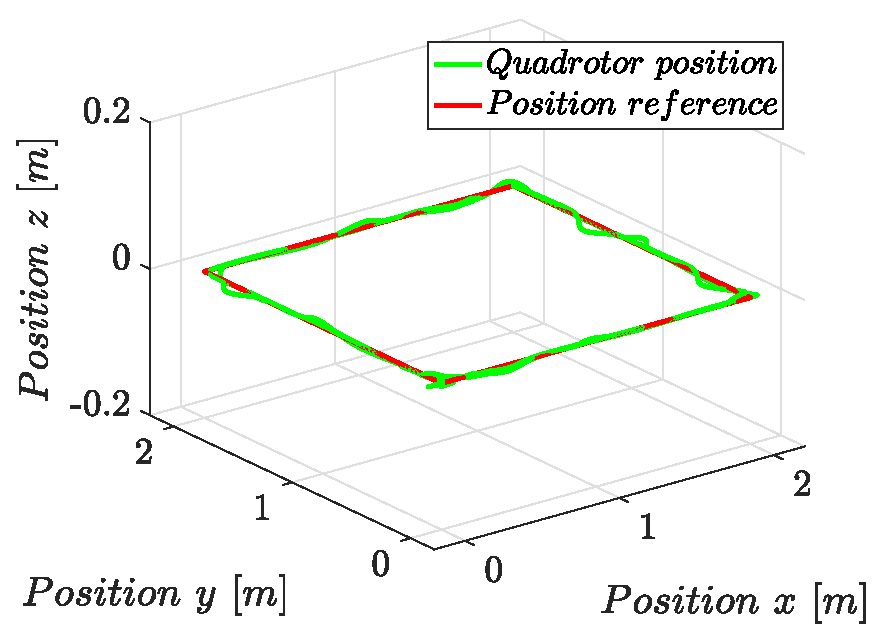
\includegraphics[width=0.8\textwidth]{auto_xyz_lqi}
	\caption{Closed-loop of the controlled system with an $H_{\infty}$ controller.}
	\label{fig:auto_xyz_lqi}
	\end{center}
	\end{figure}
	
\begin{figure}[H]
\begin{subfigure}{.5\linewidth}
\centering
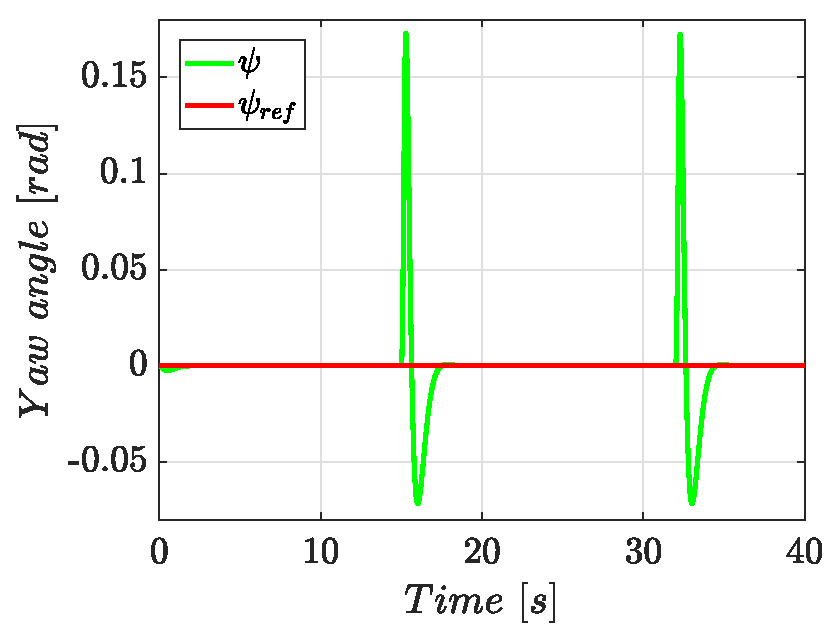
\includegraphics[width=7.0cm]{auto_psi_lqi}
\caption{Rotation about $x$ axis, $J_{xx}$ experiment}
\label{fig:auto_psi_lqi}
\end{subfigure}%
\begin{subfigure}{.5\linewidth}
\centering
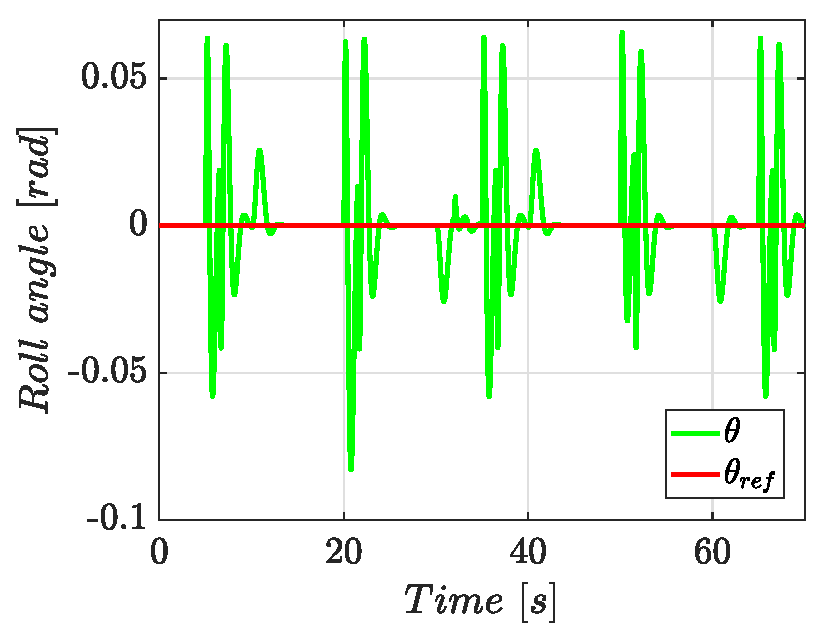
\includegraphics[width=7.0cm]{auto_theta_lqi}
\caption{Rotation about $y$ axis, $J_{yy}$ experiment}
\label{fig:auto_theta_lqi}
\end{subfigure}\\[1ex]
\begin{subfigure}{\linewidth}
\centering
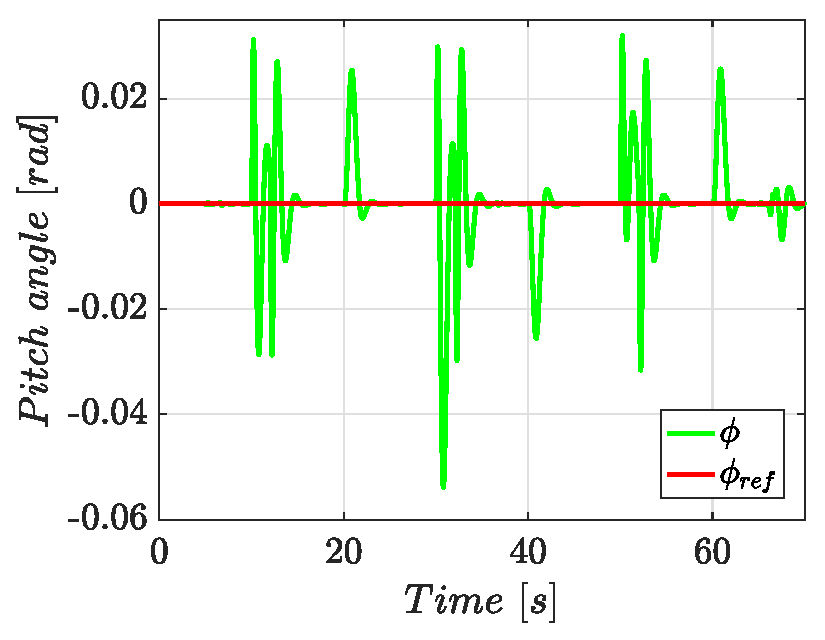
\includegraphics[width=7.0cm]{auto_phi_lqi}
\caption{Rotation about $z$ axis, $J_{zz}$ experiment}
\label{fig:auto_psi_lqi}
\end{subfigure}
\caption{Rotation about $x$, $y$ and $z$ axes during the bifilar pendulum experiments}
\label{fig:auto_lqi}
\end{figure}

\subsubsection{$H_\infty$ Controller}
rtrtererre
$\gamma = 0.5976$
\begin{figure}[h]
\begin{center}
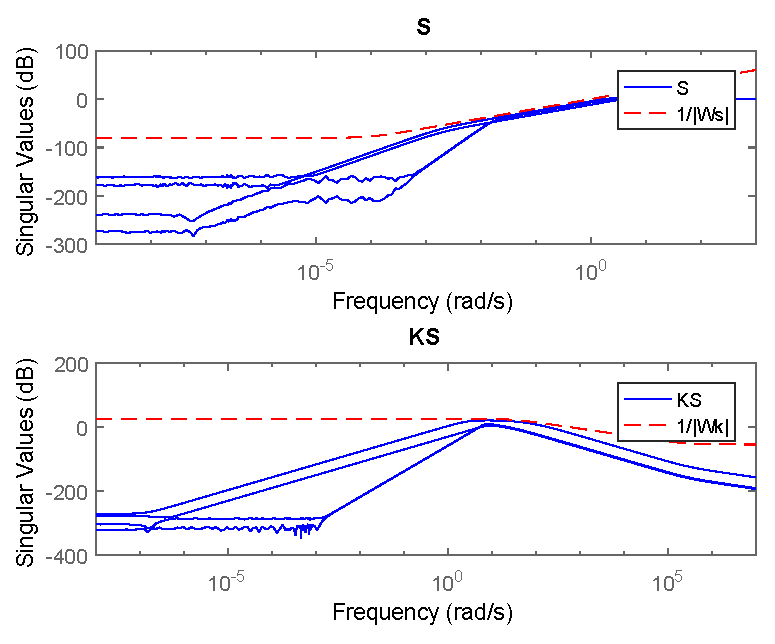
\includegraphics[width=10.8cm]{sv_auto_hinf}  
\caption{Hankel singular values energy histogram of the designed controller.} 
\label{fig:sv_auto_hinf}
\end{center}
\end{figure}

The energy of the  is shown in Fig. \ref{fig:hsv}.
\begin{figure}[h]
\begin{center}
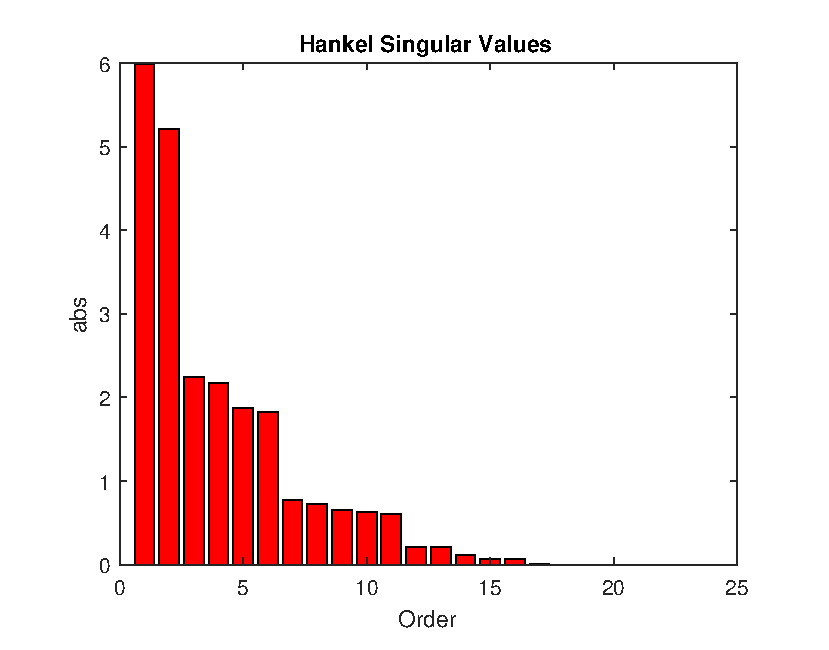
\includegraphics[width=10.8cm]{hsv_auto_h}  
\caption{Hankel singular values energy histogram of the designed controller.} 
\label{fig:hsv_auto_h}
\end{center}
\end{figure}
As shown in Fig. \ref{fig:hsv}, the last ordered four states have unnoticeable energy when it is plotted; that means that these four states can be truncated from the controller without modifying its dynamics.

\begin{figure}[h]
	\begin{center}
	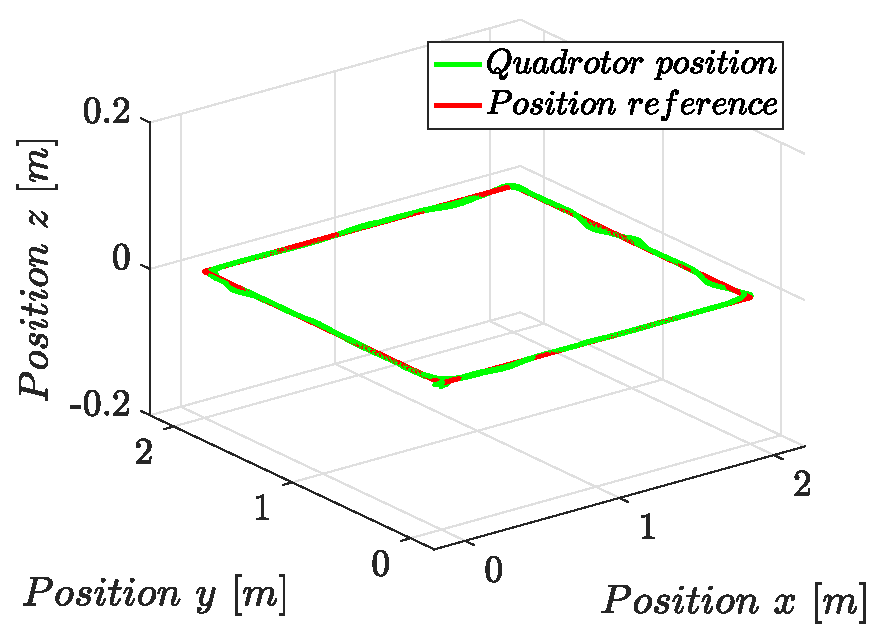
\includegraphics[width=0.8\textwidth]{auto_xyz_h}
	\caption{Closed-loop of the controlled system with an $H_{\infty}$ controller.}
	\label{fig:auto_xyz_h}
	\end{center}
	\end{figure}
	
\begin{figure}[H]
\begin{subfigure}{.5\linewidth}
\centering
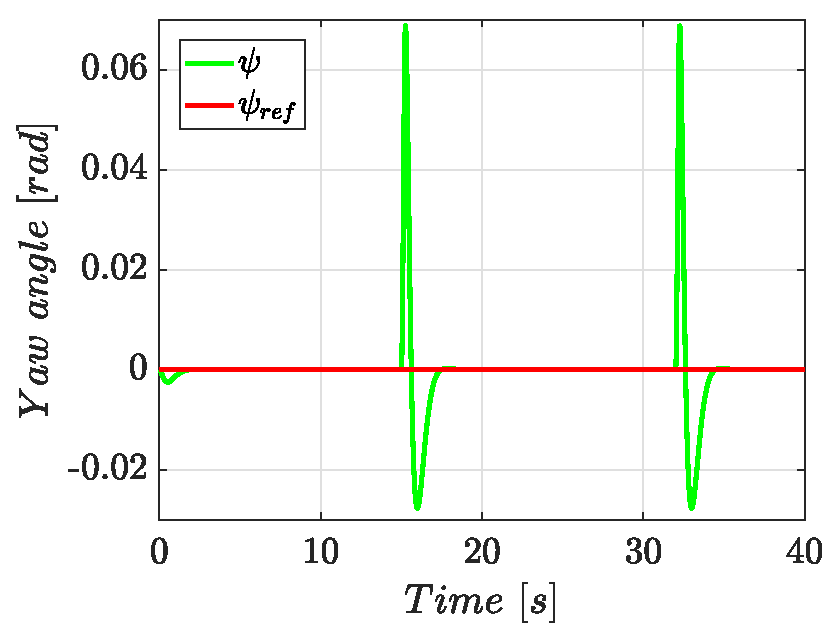
\includegraphics[width=7.0cm]{auto_psi_h}
\caption{Rotation about $x$ axis, $J_{xx}$ experiment}
\label{fig:auto_psi_h}
\end{subfigure}%
\begin{subfigure}{.5\linewidth}
\centering
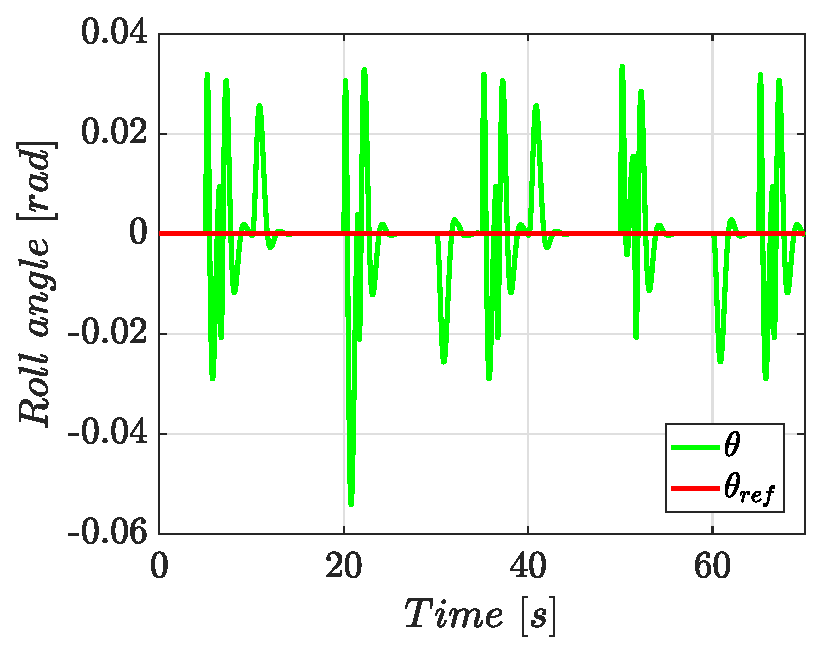
\includegraphics[width=7.0cm]{auto_theta_h}
\caption{Rotation about $y$ axis, $J_{yy}$ experiment}
\label{fig:auto_theta_h}
\end{subfigure}\\[1ex]
\begin{subfigure}{\linewidth}
\centering
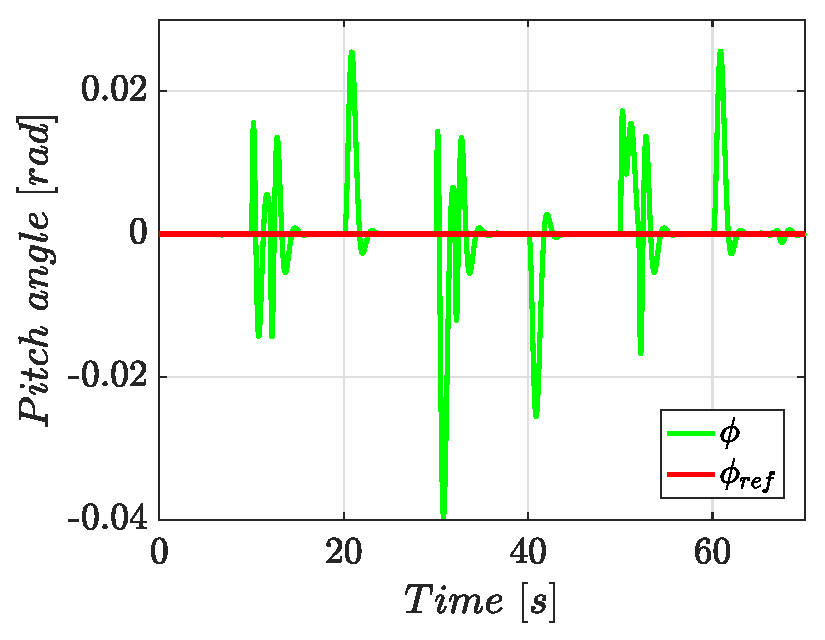
\includegraphics[width=7.0cm]{auto_phi_h}
\caption{Rotation about $z$ axis, $J_{zz}$ experiment}
\label{fig:auto_psi_h}
\end{subfigure}
\caption{Rotation about $x$, $y$ and $z$ axes during the bifilar pendulum experiments}
\label{fig:auto_h}
\end{figure}

\section{State Estimation Through Kalman Filter}
\label{sec:stateestimation}
The quadrotor dynamics are sensed exclusively using the on-board smartphone sensors. These sensors have different sample frequencies and poor accuracy. On the other hand, the LQI controller needs a full-state feedback. However, in a smartphone, it is not posible to get reliable measurements of all the components in $\mathbf{x}$. Hence, it is necessary to use estimation algorithms, as a Kalman filter, to get reliable estimations with constant sample frequency for the state vector $\mathbf{x}$.

\subsection{Attitude Estimation}
The Android API implements a Kalman filter for attitude estimation using the raw data deliverd by the smartphone accelerometer, gyroscope and magnetometer, as exposed in \cite{Astudillo2017}. Using the quaternion $Q_s$ delivered by the Rotation virtual sensor included in the Android SDK, it is obtained an absolute orientation representation with respect to the Earth frame \cite{AndSensor}, with
\begin{align}\label{eqn:rotvector}
\begin{split}
Q_{s} &= \mathrm{e}^{(\alpha/2)(u\vv{i}+v\vv{j}+w\vv{k})} \\
&= \begin{bmatrix}
\kappa_{0}\sin(\alpha / 2)\\
\kappa_{1}\sin(\alpha / 2)\\
\kappa_{2}\sin(\alpha / 2)\\
\cos(\alpha / 2)
\end{bmatrix} = \begin{bmatrix}
q_{0} \\
q_{1} \\
q_{2} \\
q_{3}
\end{bmatrix}
\end{split}
\end{align}
where $\alpha$ is the amount of degrees the quaternion is rotated around the axis $\kappa_{0}\vv{i}+\kappa_{1}\vv{j}+\kappa_{2}\vv{k}$. The rotation matrix $\mathbf{R_{b}^{w}}$ can be defined using $Q_s$ as
\begin{equation}
\label{eqn:rotbw2}
\mathbf{R_{b}^{w}} = \begin{bmatrix}
1-2(q_{2}^{2}+q_{3}^{2}) & 2(q_{1}q_{2}-q_{0}q_{3}) & 2(q_{0}q_{2}+q_{1}q_{3}) \\
2(q_{1}q_{2}-q_{0}q_{3}) & 1-2(q_{1}^{2}+q_{3}^{2}) & 2(q_{2}q_{3}+q_{0}q_{1}) \\
2(q_{1}q_{3}+q_{0}q_{2}) & 2(q_{0}q_{1}+q_{2}q_{3}) & 1-2(q_{1}^{2}+q_{2}^{2})
\end{bmatrix}.
\end{equation}
Comparing (\ref{eqn:rotbw1}) and (\ref{eqn:rotbw2}), the Euler angles ($\psi_{m}$, $\theta_m$, $\phi_m$) are then obtained from the quaternion $Q_s$ as
\begin{equation}\label{eqn:quattoeu}
\begin{bmatrix}
\psi_{m} \\
\theta_{m} \\
\phi_{m}
\end{bmatrix} =
\begin{bmatrix}
atan2(2(q_{3}q_{2} + q_{0}q{1}),1-2(q_{1}^{2} + q_{2}^{2})) \\
arcsin(2(q_{3}q_{1} - q_{2}q_{0})) \\
atan2(2(q_{3}q_{0} + q_{1}q{2}),1-2(q_{0}^{2} + q_{1}^{2})) 
\end{bmatrix}.
\end{equation}

\subsection{Position Measurement}
The smartphone used in this project, can measure its position with respect to the Earth-frame. For this task, it counts with a GNSS receiver and a barometer.
The $x_{m}$ and $y_{m}$ position measurements, with respect to the $X_W$ and $Y_W$ axes, are acquired using the GNSS receiver. 
\\\\
Each coordinates sample is initially set in an ellipsoidal representation of decimal degrees, following the WGS84 coordinate system. Then, the coordinates are converted to a bi-dimensional representation in meter units using the cartographic projection Magna-Sirgas (projection EPSG:3115).
\\\\
The altitude measurements $z_{m}$ are acquired using the barometric pressure sensor which delivers the pressure value $p_k$ in hPa units. This signal is converted to meters as
\begin{equation}\label{eqn:hbarom}
z_{m} = 44330\left(1-\frac{p_k}{p_{0}}^{1/5.255}\right)\ [m],
\end{equation}
where $p_{0}$ is the atmospheric pressure at sea level \cite{Lauszus2015}.
\\\\
The smartphone GNSS receiver and barometer were tested statically, leaving the phone in a stable position for 100 minutes, with an ambient temperature of $22\ ^{\circ}C$ and a UV index of $3$. The results of the test are shown in Fig. \ref{fig:sensorstest}
\begin{figure}[h]
\begin{subfigure}{.5\linewidth}
\centering
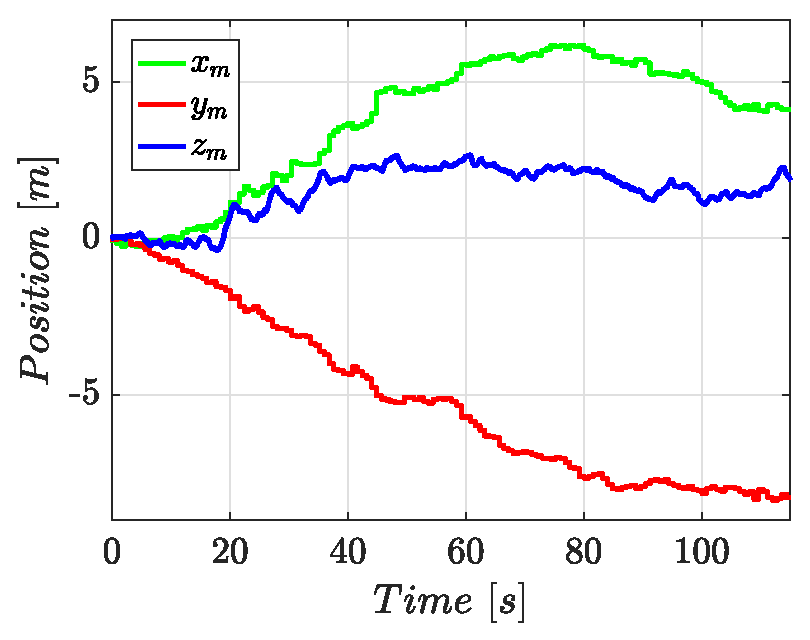
\includegraphics[width=7.0cm]{pos_test}
\caption{Position drift}
\label{fig:pos_test}
\end{subfigure}%
\begin{subfigure}{.5\linewidth}
\centering
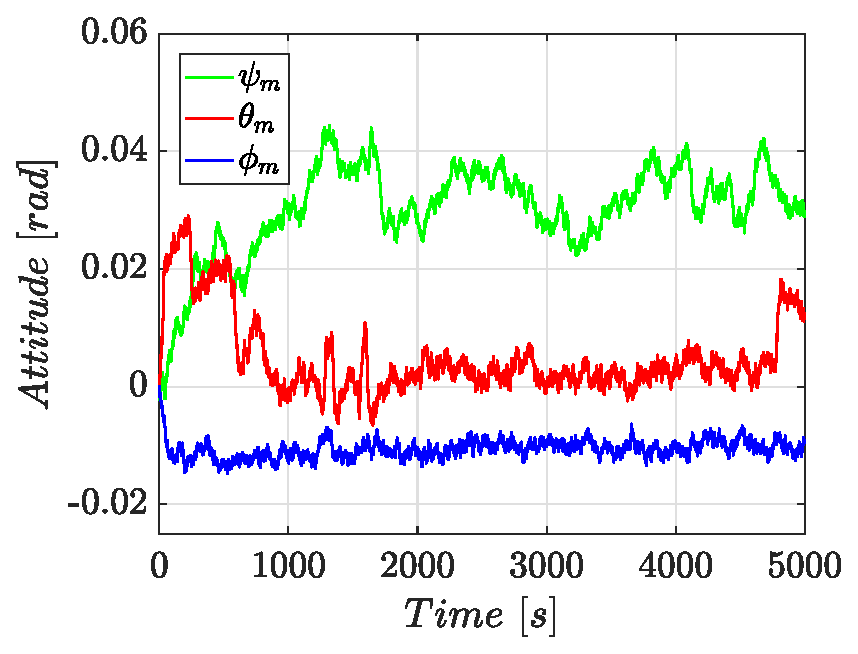
\includegraphics[width=7.0cm]{att_test}
\caption{Attitude drift}
\label{fig:att_test}
\end{subfigure}\\[1ex]
\begin{subfigure}{\linewidth}
\centering
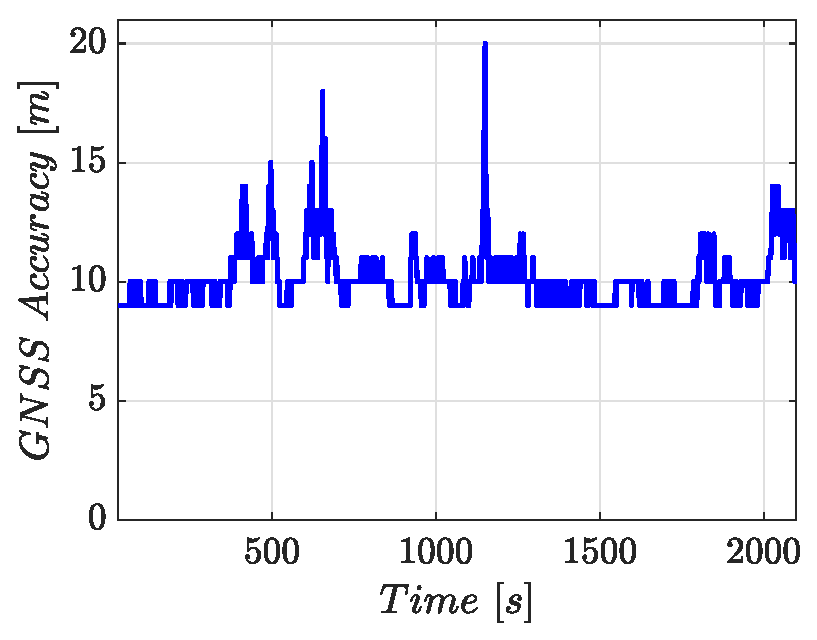
\includegraphics[width=7.0cm]{gpsacc_test}
\caption{GNSS receiver accuracy}
\label{fig:gpsacc_test}
\end{subfigure}
\caption{Results of the static test of the smartphone GNSS receiver and barometer}
\label{fig:sensorstest}
\end{figure}
\\\\As seen in Fig. \ref{fig:pos_test}, even though the phone was kept in a static position, the $x_m$ and $y_m$ position signal received from the GNSS receiver shows a change of about $6\ m$ in both the $X_W$ and $Y_W$ directions, after just $60\ s$. The $z_m$ position, however, has sudden changes in short periods of time, but without reaching errors greater than $2.5\ m$. The attitude results, Fig. \ref{fig:att_test}, show stable signals for the three Euler angles. The $\psi_m$ and $\theta_m$ angles suffer from a drift of about $0.04$ and $-0.02\ rad$ respectively, while the initial drift suffered by $\phi_m$ is just $-0.01\ rad$.
\\\\
Despite being under a clear sky, where the smartphone could have visibility of more than six satellites of the GPS and GLONASS constellations, the GNSS accuracy value, delivered by the receiver in the smartphone, is always more than $9\ m$ as seen in Fig. \ref{fig:gpsacc_test}. 
\\\\
\subsection{States Estimation}
In order to estimate all the components of the state vector $\mathbf{x}$, a Kalman filter is designed. The Kalman filter is an iterative algorithm that estimates the observable (and not measurable) states of a system, using the measurable variables, the inputs and the variances of the noises that affect the system.
\\\\
This filter is designed using the linearized dynamic model of the quadrotor from Section \ref{sec:linearized}, where $\mathbf{x} =  \begin{bmatrix}
x & \dot{x} & y & \dot{y} & z & \dot{z} & \psi & \dot{\psi} & \theta & \dot{\theta} & \phi & \dot{\phi}
\end{bmatrix}^{T}$, and using the discretized representation $\mathcal{G}_k$.
\\\\
The algorithm starts calculating a prediction of the state $\hat{\mathbf{x}}_{k}^{-}$ and its covariance $P_{k}^{-}$ as
\begin{equation}\label{eqn:statePrognosis}
\hat{\mathbf{x}}_{k}^{-} = A_k\hat{\mathbf{x}}_{k-1}+B_k\mathbf{u},
\end{equation}
\begin{equation}\label{eqn:covariancePrognosis}
P_{k}^{-} = A_k P_{k-1} A_{k}^{T} + Q_{k},
\end{equation}
where $\hat{\mathbf{x}}_{k-1} = \hat{\mathbf{x}}(k-1)$ is the previous estimated state, $P_{k-1}$ the previous error covariance matrix and $Q_{k}$ the process variance. The state prediction is then corrected using the Kalman gain vector
\begin{align}\label{eqn:correctionKalman}
\begin{split}
K_{k} &= P^{-}_{k}H^{T}(HP^{-}_{k}H^{T} + R_k)^{-1},
\end{split}
\end{align}
and updating the state estimation $\hat{\mathbf{x}}_{k}$ and its covariance $P_{k}$, based on the measurements $\vartheta_k$ as
\begin{align}\label{eqn:correctionKalman2}
\begin{split}
\hat{\mathbf{x}}_{k} &= \hat{\mathbf{x}}^{-}_{k} + K_{k}(\vartheta_{k} - H\hat{\mathbf{x}}^{-}_{k}),\\
P_{k} &= (\mathcal{I} - K_{k}H)P^{-}_{k},
\end{split}
\end{align}
where $R_k$ is the measurement covariance matrix, $\mathcal{I}$ is the identity matrix and $H$ is the matrix that satisfies
\begin{equation}
\vartheta_k = H \mathbf{x}_k.
\end{equation}
The measurements vector $\vartheta_k$ is set as
\begin{equation}
\vartheta_k = \begin{bmatrix}
x_{m} & y_{m} & z_{m} & \psi_{m} & \theta_{m} & \phi_{m}
\end{bmatrix}^{T},
\end{equation}
so matrix $H$ is defined as
\begin{equation}\label{eqn:H}
H =\begin{bmatrix}
1 & 0 & 0 & 0 & 0 & 0 & 0 & 0 & 0 & 0 & 0 & 0\\
0 & 0 & 1 & 0 & 0 & 0 & 0 & 0 & 0 & 0 & 0 & 0\\
0 & 0 & 0 & 0 & 1 & 0 & 0 & 0 & 0 & 0 & 0 & 0\\
0 & 0 & 0 & 0 & 0 & 0 & 1 & 0 & 0 & 0 & 0 & 0\\
0 & 0 & 0 & 0 & 0 & 0 & 0 & 0 & 1 & 0 & 0 & 0\\
0 & 0 & 0 & 0 & 0 & 0 & 0 & 0 & 0 & 0 & 1 & 0
			\end{bmatrix}.
\end{equation}
This algorithm is executed once every sampling period, after which, the controller can use the vector of estimated states $\hat{\mathbf{x}}_{k}$ as feedback.



\section{Conclusions}
This chapter presented the simulation and the testing of five control techniques
for the attitude control of a quadrotor. The first technique is based
on Lyapunov theory, it proved to be very reactive, especially for the yaw
angle control. However, the stabilization in the direct neighborhood of the
equilibrium point was not rigid enough to permit hover flight. The second
one is a PID controller, it proved to be well adapted to the quadrotor when
flying near hover. It was possible using this technique to successfully perform
the first autonomous flight. The PID controller was only able to control the
quadrotor in near hover and absence of large disturbances. The third one
is an LQ controller, it displayed average stabilization results. It showed to
be less dynamic than the PID. The fourth control technique is the Backstepping,
its ability to control the orientation angles in presence of relatively
high perturbations is very interesting. The sliding-mode technique is the fifth
approach, it did not provide excellent results. The switching nature of the
controller seems to be ill adapted to the dynamics of the quadrotor. The results
of all these control approaches conducted to a combination of PID and
Backstepping into the so-called Integral Backstepping. This was proposed
as a single tool to design attitude, altitude and position controllers. The
experiment has shown that OS4 is currently able to take-off, hover, land and
avoid collisions automatically. As far as we know, OS4 is the first quadrotor
practically capable of a collision avoidance maneuver.
